\chapter{ILLUMINATION-ROBUST VISUAL LOCALIZATION AND MAPPING}

\section{Introduction}

In recent decades, real-time \acrshort{vslam}/\acrshort{vo} systems have shown their full potentials to assist various outdoor robotic applications, especially in the field of autonomous driving for urban and suburban operations.  
However, few of them have been successfully demonstrated in unstructured natural environments.
In general, the use of indirect methods is prohibited by their degraded feature matching performance due to the significantly increased environmental complexity. 
Such degeneration can turn into a vicious circle: the decreased inlier/outlier ratio will result in a reduced amount of landmarks maintained in the map, which, in turn, makes the 3D-2D registration more fragile.   
To solve this problem, indirect systems usually propose to involve more points or more capable descriptors into the data association pipeline.
However, it often comes at the price of unjustified computational expense that eventually prevents their real-time operations. 

In contrast, direct methods can easily incorporate more keypoints in the estimation process without significant computational overheads. 
It is achieved through directly comparing the intensity value of pixels over a local patch across images by making a brightness constancy assumption. 
However, it also brings out some issues to be deliberately addressed:
\begin{enumerate}
	\item The highly efficient loose data association strategy comes at the price of the sensitivity to unmodeled photometric disturbance, where the outdoor images often suffer from such uncertainties, e.g. camera over-exposures, smooth lighting changes, and even solar flares, as shown in \ref{fig:illumination_typicalnoise}. 
	\item The non-smoothness nature of the image makes the direct image alignment problem very sensitive to the initial condition during optimization.
Although the image-pyramid-based coarse-to-fine direct alignment strategy has proven to alleviate the non-convexity of the problem, the convergence basin is still greatly compromised.
Worse still, the illumination-robust direct energy functions usually achieve lighting change invariance by discarding the low-frequency components of the image, which makes the situation more severe. 
\end{enumerate}

\begin{figure}[t] 
  	\centering
  	\includegraphics[width=\linewidth]{figures/illumination/typical_lighting_changes.pdf}
    \caption[Typical Lighting Changes in Natural Environments]{ \textbf{Typical Lighting Changes in Natural Environments.} Local and global lighting changes are abundant in natural images \cite{griffith2017symphony}. The example 3D reconstruction is presented in (a), and two pairs of example images with global illumination changes in (b) and two pairs with local+global illumination changes in (c) are illustrated. 
	\label{fig:illumination_typicalnoise}}
\end{figure}

Besides the illumination-robust cost functions, edges are alternatives to point features with improved robustness to the aforementioned situations. 
Specifically, edges are geometric features extracted from raw images with inter-frame edge registration performed using \acrlong{icp} (\acrshort{icp}) based direct alignment \cite{kneip2015sdicp} \cite{zhou2017semi} \cite{zhou2018canny}.
Such binarization and \acrshort{icp}-based registration theoretically decouple the illumination-sensitive components from the edge features, thus be more suitable for lighting challenging situations. 
Thanks to the recent development of edge detection algorithms, the repeatability of edges across images have been significantly improved even under rapid lighting changes, which laid the foundation of the edge \acrshort{vslam}/\acrshort{vo} applications. 
However, there are also some bottlenecks to implement edge feature in monocular \acrshort{vslam}/\acrshort{vo}:
\begin{enumerate}
	\item Binary edge features usually lead to partially observable depth under \acrshort{icp}-based mapping frameworks. 
Conventional depth estimation algorithms that search for best matches along Epipolar lines may result in unreliable correspondences and lead to unstable and error-prone depth estimates in \ref{fig:illumination_edgedeficiency}. 
Such deficiency pre-close the feasibility to incorporate edge features in the joint optimization process of monocular \acrshort{vslam}/\acrshort{vo}. 
\end{enumerate}

\begin{figure}[t] 
  	\centering
  	\includegraphics[width=\linewidth]{figures/illumination/edge_deficiency.pdf}
    \caption[Deficiency of Edge Mapping]{\textbf{Deficiency of Edge Mapping.} The desired edge mapping algorithm (\textbf{Top}) is capable of overcoming the partial observability issue of pure Edge Mapping (\textbf{Bottom-Left}), where the pure edge mapping minimize point-to-tangent error ({\color{green!50!black} $\uparrow$}) that results in more erroneous matches ({\color{red} $\blacksquare$}) under poorly-observable direction (\textbf{Bottom-Right}) than observable direction (\textbf{Bottom-Mid}).
    \label{fig:illumination_edgedeficiency}}
\end{figure}

In this chapter, we focus on three key developments towards the above-mentioned problem: 
\begin{enumerate}
	\item \textbf{Illumination-Robust Direct \acrshort{vo}} The illumination-invariant costs that have shown excellent performance in indoor evaluations is revisited in the context of monocular joint optimization framework \cite{engel2018direct} in the outdoor environment.
Based on the analysis, a combined cost that adaptively weights a global affine model-based cost and a gradient-based cost in different optimization phases are proposed to achieve high-precision motion estimation, while preserving a large convergence basin.
	\item \textbf{Illumination-Robust Edge \acrshort{vo}} A monocular edge \acrshort{vo} framework, comprised of \acrshort{icp}-based edge alignment, edge-guided data association, and local \acrshort{ba}, which is capable of performing illumination-robust camera tracking and scene reconstruction without incurring edge mapping degradation.  
An edge-guided data association pipeline incorporating probabilistic search length approximation, image-gradient-based template matching, match-confidence-based patch size adaption, and depth-confidence-based match conditioning.
A point-to-edge geometric uncertainty analysis that analytically derives a probabilistic search length formula and a depth confidence measure that improves the efficiency and accuracy of our proposed system.
	\item \textbf{Semantics-Aided Edge \acrshort{vo}} As an extension of edge \acrshort{vo}, a semantic edge \acrshort{vo} framework is proposed to reconstruct large-scale semantic maps in challenging outdoor environments. The core of this approach is a semantic nearest neighbor field that facilitates a robust data association of edges across frames using semantics. This significantly enlarges the convergence radius during tracking phases.  
\end{enumerate}

\section{Background}

\noindent \textbf{Illumination-Robust Direct \acrshort{vslam}/\acrshort{vo}} In recent years, a number of illumination-robust \acrshort{vslam}/\acrshort{vo} systems have been proposed, implementing various models or descriptors to alleviate the adverse effect of external lighting changes, so as to achieve robust motion estimation in challenging indoor and outdoor environments. To gain robustness against the global illumination changes, either the median value of pixel residuals \cite{meilland2011real} \cite{gonccalves2011real} \cite{bloesch2015robust} \cite{greene2016multi} or an affine brightness transfer function \cite{klose2013efficient} \cite{engel2015large} is estimated to compensate the induced adverse effect in the optimization. For local lighting changes, \cite{dai2017bundlefusion} propose to use image gradients, rather than pixel intensities, to formulate the direct energy function, thus gaining local lighting invariance; \cite{crivellaro2014robust} relies on dense computation of a deliberately designed local descriptor to obtain a clear global minimum in energy function while preserving convergence basin by convolving with a low-pass filter; the methods based on the census transform \cite{alismail2016direct} use a binary descriptor to achieve local illumination invariance during the motion estimation. 

A thorough evaluation regarding accuracy and robustness in the context of visual odometry is conducted for all described methods above in \cite{park2017illumination}. The analysis results suggest that the gradient-based method\cite{dai2017bundlefusion} and census-transform-based method \cite{park2017illumination} show state-of-the-art performances. However, all the methods and their evaluations are conducted with RGB-D and stereo setup, where the depth information is provided with some precision.

\noindent \textbf{Edge \acrshort{vslam}/\acrshort{vo}} The first edge \acrshort{vo} \cite{jose2015realtime} aligned edges by searching for the closest counterpart along the normal direction.  Later, efficiency improvements for 2D-3D registration based on the \acrlong{dt} (\acrshort{dt}) \cite{kneip2015sdicp} improved the real-time properties of motion estimation. The optimizability of this formula is further improved by substituting DT with \acrlong{annf} (\acrshort{annf}) \cite{zhou2017semi} or \acrlong{onnf} (\acrshort{onnf}) \cite{zhou2018canny}, which have demonstrated strong performances for RGB-D sensors. For RGB-D sensors these techniques work well. Meanwhile, image-only monocular edge-based \acrshort{vo} remains challenging since binary
edge features lead to partially observable depth under \acrshort{icp}-based mapping frameworks. 

To address the partial observability issue of edge mapping, more sophisticated group matching strategies can realize geometrically consistent matches \cite{tarrio2019se}, but fail to provide any theoretical guarantees on correctness. Using optical flow \cite{bouguet2001pyramidal} to find the matches through photometric minimization makes the depth fully observable in the back-end \cite{maity2017edge}. However, most optical flow methods rely on the brightness constancy assumption, limiting the set of situations for which edges complement point features. %its use for outdoor operations. 

\noindent \textbf{Semantics-Aided \acrshort{vslam}/\acrshort{vo}} With the recent advances in deep learning, semantic information has become relevant for motion estimation.  \cite{yu2018ds} \cite{mahe2018semantic} use semantics to detect moving objects and alleviate their pixels weights in the objective function.  Similarly, \cite{kaneko2018mask} masks the sky pixels. \cite{lianos2018vso} integrates a semantic reprojection error into existing point-based indirect and direct motion estimation systems. The overall advantage of integrating semantics is to boost the tracking and mapping robustness and accuracy. We pursue these efforts and fuse the advantages from both semantic-\acrshort{vslam} and learned-edges-\acrshort{vslam} to make \acrshort{vo} even more robust.

\noindent \textbf{Deep Learned Edges} Previous edge-based SLAM methods rely on the standard Canny edge detector \cite{canny1987computational}, but \cite{schenk2017robust} shows that using machine-learned edges \cite{dollar2015fast} \cite{xie2015holistically} gives significant improvements compared to standard edges in indoor settings. Structured edges (SE) \cite{dollar2015fast} generalizes random forests to general structured output spaces to learn edges on patch images. Despite its fast computation time, it relies on hand-crafted features and requires to map the ground-truth edges to low dimensional representation for the training to be scalable. These drawbacks are alleviated with the deep-learning based HED \cite{xie2015holistically}: it processes raw images and outputs an edge probability map over the input in the form of a binary map. In this work, we extend edge-based \acrshort{vslam} and enhance them with semantic information to make them more robust. To do so, we use learned-edges together with their semantic labels as computed in \cite{yu2017casenet} \cite{yu2018simultaneous}.
CaseNet \cite{yu2017casenet} extends HED \cite{xie2015holistically} to multi-label edges and outputs a distinct probability edge map for each semantic class.  SEAL \cite{yu2018simultaneous} continues the efforts of \cite{yu2017casenet} and tackles the challenge of edge-alignment during the \acrshort{cnn} training. Label noise in the human-annotated ground-truth edges leads CaseNet to learn thick edges which hides relevant edges details. However, none of these works investigate the application of semantic edges in \acrshort{vo}. In contrast, we provide a method to integrate any semantic edge into \acrshort{vo} and run extensive experiments to compare the influence of edge and semantic learning on the \acrshort{vo} performances.
 
\section{Datasets}

The overall system performance of our proposed edge \acrshort{vo} algorithm is evaluated using Symphony Lake \cite{griffith2017symphony} dataset, which consists of millions of natural lakeshore images heavily contaminated by (1) smooth (auto-exposure) and (2) sudden (sun-glares) lighting changes, as well as (3) the tree-sky boundary pixel over-exposure in \ref{fig:illumination_typicalnoise}. Unlike sun-glares that randomly occurs in sunny days of a year, the over-exposure induced appearance changes show significant variations across seasons. In general, the denser the leaves in Summer, the fewer boundary pixels are 'eaten' by lights the \acrshort{vo} system is, therefore, less affected by over-exposure, and the opposite holds in Winter. Based on these observations, we choose 12 surveys (3 surveys per season) heavily contaminated with sun-glare and categorize results based on seasons. For motion robustness evaluation, we down-sample the selected sequences at a sample rate of 3 for fast camera motion simulation. For quantitative analysis, the ground truth pose is calculated through Laser-GPS-based global pose graph optimization described in \cite{pradalier2018multi}. The scale of trajectory from monocular \acrshort{vo} are corrected using ground truth poses at every 200 frames, while the loop-closure functionality is disabled for ORBSLAM2 \cite{mur2017orb} for a fair comparison.

Another outdoor dataset used in this section is one of the most famous autonomous driving dataset KITTI \cite{geiger2012we}.  
The odometry benchmark of KITTI consists of 11 stereo sequences with ground truth trajectories calculated from a Velodyne laser scanner and a \acrshort{gps} localization system.
The stereo images used in this section are captured from two high-resolution video cameras by driving around the mid-size city of Karlsruhe, in rural areas and on highways, where the basic information is summarized in \ref{tbl:kitti_dataset}. 
Compared to Symphony Lake Datasets, KITTI datasets presents significantly less rapid lighting changes and sharp camera motions, thus being considered as less challenging outdoor datasets for evaluation. 

\begin{table}[h]
	\centering
	\caption[Dataset Information]{ Dataset Information
	\label{tbl:kitti_dataset}}
	\begin{tabular}{ccc}
\hline
Scene   & Sequence No.        & Description                              \\ \hline
city    & 00, 05, 06, 07      & buildings, cars with few vegetation  \\
village & 02, 03, 04,  08, 09 & vegetation with few buildings, cars \\
highway & 01                  & roads, cars, and signs                   \\ \hline
	\end{tabular}
\end{table}

\section{Illumination-Robust Direct VO}
\label{sec:illumination_direct}

In this section, an illumination-robust direct monocular SLAM system that focuses on modeling outdoor scenery is presented. 
To deal with global and local lighting changes, such as solar flares, the state-of-art illumination invariant photometric costs for RGB-D and stereo \acrshort{vslam} systems are revisited in the context of their monocular counterpart, where the camera motion and scene structure are jointly optimized with a reasonably poor initialization. 
Based on our analysis, a combined cost is proposed to achieve a high-precision motion estimation with an improved convergence radius. 
The proposed system is extensively evaluated on the synthetic and real-world datasets regarding accuracy, robustness, and processing time, where our approach outperforms systems with other costs and state-of-art DSO and ORBSLAM2 systems.

\subsection{Illumination-Robust Costs}

Instead of presenting all real-time capable illumination-invariant formulations suitable for the joint optimization framework, we merely present methods that achieved excellent performances in \cite{park2017illumination}. 
The intensity values of the grayscale image is utilized to serve as a baseline method. 
The global affine model is estimated to compensate the global lighting changes.
The gradient magnitude is used to formulate energy function thus achieving invariance to local illumination change.
The local descriptor from \cite{alismail2017direct}, named Census Transform or bit-plane, is presented to achieve local illumination invariance. 

\subsubsection{General Photometric Energy Function}

Recall the generalized photometric energy function described in \ref{eq:preliminaries_photometricerror}:
\begin{equation} \label{eq:illumination_photometric}
E_{kr}^{\mathcal{P}} := \sum_{\mathbf{p}_r \in \mathit{S}_r^{\mathcal{P}}} w_{\mathbf{p}_r}^{\mathcal{P}} \Vert F_{k} ( \mathbf{p}_{kr}) - F_{r}(\mathbf{p}_r) \Vert_{\gamma}  
\end{equation} 
where $F(\cdot)$ represents the representation calculated from the raw image.  
All the mentioned approaches can be seen as specifications or simple extensions of such formulation. 

\subsubsection{Intensity}
For standard implementation \cite{engel2018direct}, we model the unknown function $F(\cdot)$ as an image function mapping 2D pixel coordinate to pixel intensity values obtained by bilinear interpolation, where a mathematical expression can be written as:
\begin{equation} \label{eq:illumination_intensity}
F_{Int}(\cdot) := I(\cdot)
\end{equation}
As the standard implementation, the intensity-based method serves as a baseline approach for comparison.

\subsubsection{Global Affine Model}
The global affine model in \cite{klose2013efficient} \cite{engel2015large} can be plugged into the basic direct formulation, in \ref{eq:illumination_photometric}, to compensate for the additive and multiplicative global lighting or exposure changes, where the pixel-wise energy function can be modified as: 
\begin{equation} \label{eq:illumination_affine}
E_{kr,GAff} :=  \sum_{\mathbf{p}_r \in \mathit{S}_r^{\mathcal{P}}} w_{\mathbf{p}_r}^{\mathcal{P}} \Vert F_{k} ( \mathbf{p}_{kr})  - \beta_k - \frac{e^{\alpha_k}}{e^{\alpha_r}} F_{r}(\mathbf{p}_r) - \beta_r \Vert_{\gamma}  
\end{equation}
where $\alpha_{k,r}$ and $\beta_{k,r}$ are global illumination affine model parameters, which are jointly optimized at each iteration. Combined with Huber norm, this {\em affine} method can work well in an environment without substantial local illumination changes.

\subsubsection{Gradient Magnitude}
In \cite{dai2017bundlefusion}, the gradient magnitudes are utilized, instead of intensities, to formulate unknown function $F(\cdot)$ with a mathematical expression as:
\begin{equation} \label{eq:illumination_gradient}
F_{Grad}(\cdot) :=  \Vert \nabla I(\cdot)\Vert_{2}
\end{equation}
where $\nabla I(\cdot)$ calculates the gradient vector from the image intensities around a given pixel. The {\em gradient} method has proven to be robust with the local lighting changes and could achieve state-of-art tracking precision for RGB-D and Stereo applications. 

\subsubsection{Census Transform}
\label{sec:census}
The Census Transform \cite{alismail2016direct} is a local binary descriptor that compares a pixel intensity with its neighborhoods and results in one-bit results indicating the neighbors are lighter or darker than this given pixel. The results are then packed to formulate the bit-plane descriptor, which is the $F(\cdot)$ in this work. Considering a $N \times N$ local patch is utilized to calculate the descriptor, where the $i^{th}$ descriptor can be written as:
\begin{equation} \label{eq:illumination_ct}
F_{CT}(\cdot) :=  \sum_{i \in \mathcal{N}} 
\begin{cases}
    1,              & \text{if } I(\cdot) > I(N_i(\cdot))\\
    0,              & \text{otherwise}
\end{cases}   
\end{equation}
where $N$ represent the neighborhoods of the given pixel. It should be noted that the choice of the comparison operator is flexible, which could be $>$, $\leq$, $<$, or $\geq$, but it must be consistent for all pixels of interest. The gradient of the descriptor is approximated by using its image gradient for Jacobian computation in optimization.

\subsection{Convergence-Preserved Joint Optimization}

Ultimately, an adaptively combined cost, using both an intensity-based energy with a global affine model and gradient-based energy, is proposed to achieve the invariance against global and local lighting changes without compromising convergence robustness.   

\begin{figure}[t] 
  	\centering
  	\includegraphics[width=0.8\linewidth]{figures/illumination/direct_energy_function.pdf}
	\caption[Example Energy Functions under Different Lighting Conditions]{ \textbf{Example Energy Functions under Different Lighting Conditions.} The pixel-wise energy function of each described method is plotted against the pixel depth in four lighting conditions: (a) no illumination changes, (b) local illumination change, (c) global illumination change, and (d) local and global illumination change. 
	\label{fig:illumination_energyfunc}}
\end{figure} 

From the analysis of tracking accuracy and the convergence radius, we found that the {\em gradient} method showed maximum robustness against various simulated lighting changes over other methods. However, it has a smaller convergence radius compared with the {\em affine} approach. 

Motivated by descriptor field method \cite{crivellaro2014robust}, we propose to combine the energy functions of {\em affine}, and {\em gradient} approaches to obtain a clear global minimum while preserving large convergence basin through an adaptively re-weighted optimization strategy. The idea behind adaptive weighting strategy is assigning weights to {\em affine} and {\em gradient} costs at the different stage of the optimization: more weights put on the {\em affine} component at the beginning of optimization and more on the {gradient} component at the end. In practice, we achieve this by re-estimating $w_k$ when the total energy arrives at the local minimum during optimization. Mathematically, the proposed pixel-wise energy can be expressed as:  
\begin{equation} \label{eq:illumination_combined}
E_{kr} :=  (1-w_{kr}) E_{kr,GAff} +\frac{1}{2 \sqrt{2} } w_{kr} E_{kr,Grad} 
\end{equation}
where the $2 \sqrt{2}$ is the factor that scales the gradient magnitude to be the same range with intensity, which is set as the maximum value ratio between intensity and gradient magnitude. The $w_k$ is the adaptive weight that starts from 0 and ends up with 1, which can be defined differently in the tracking phase $w_{k,1}$ and reconstruction phase $w_{k,2}$ as: 
\begin{equation} \label{eq:illumination_reweight}
w_{k,1} :=  \frac{1}{tr({\Sigma}_{\xi})} \quad w_{k,2} :=  \frac{1}{\sigma^2_{d^{-1}_k}}
\end{equation}
where $tr(\cdot)$ represents the trace operator, ${\Sigma}_{\xi}$ is the covariance matrix of pose estimates, and $\small \sigma^2_{d^{-1}_k}$ is the variance of inverse depth of the pixel from joint optimization. 

In the tracking phase, the inverse depth of pixel is set constant, and the camera pose is the only parameter to be optimized so that the measure of pose estimate uncertainty weights the costs. In the reconstruction phase, the camera poses are already well-initialized, and the inverse depth estimates play a more critical role in the joint optimization, where the inverse depth uncertainties balance two costs to facilitate a robust estimation. As a result, the uncertainty based weights, $w_{k,1}$ $w_{k,2}$, could force the estimate with a huge amount of uncertainty to have a large convergence basin and guide the determinate estimate to arrive at the global minimum, thus improving the tracking precision and robustness. 

The formulated pixel-wise energy function is analyzed in four typical lighting conditions in \ref{fig:illumination_energyfunc}. In the comparison of all other methods, our proposed method holds nice cost functions in all conditions: a clear global minimum and large convergence basin. Note that this analysis uses the real-world image with simulated illumination changes, so that the costs in {\em const} mode can serve as the ground truth values. 

\subsection{Evaluation}
In this section, The tracking accuracy and convergence radius during tracking phase are quantitatively evaluated and compared for each described methods, and their overall system performance analysis regarding tracking accuracy, robustness, and runtime properties are presented. 
Besides, a qualitative evaluation is performed to study the effect of solar glare on our proposed system to further support our claims.
  
\subsubsection{Tracking Accuracy and Convergence Radius }

\begin{figure}[t] 
	\centering
	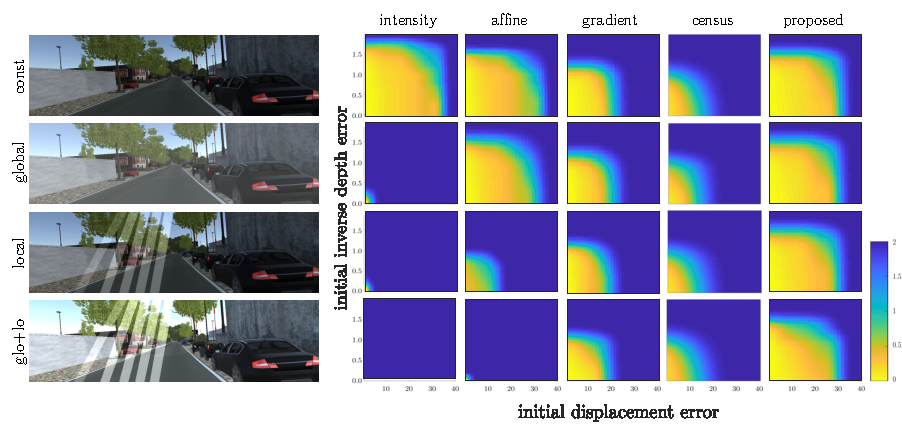
\includegraphics[width=\linewidth]{figures/illumination/direct_convergence_test.pdf}
	\caption[Evaluation of Convergence Basin]{\textbf{Evaluation of Convergence Basin.} \textbf{Left}: the example images with simulated illumination changes are provided in four lighting conditions: no lighting changes, global lighting changes, local lighting changes, and global+local lighting changes. \textbf{Right}: the tracking errors are plotted versus initial pose displacement (x-axis) and maximum inverse depth error (y-axis) for each described methods in different conditions. 
	\label{fig:illumination_convergence}}
\end{figure}

The tracking accuracy and the convergence radius, in the tracking phase, are quantitatively evaluated using synthetic vKITTI dataset, where both ground truth pose and depth map are provided. 
The images are pre-processed to add the global illumination bias or/and solar-glare patterned local illumination changes with the value ranging from $-20$ to $+20$. 
To prepare the inverse depth map as initialization, the ground truth depths are first mapped to inverse depths and normalized to average $1.0$, and the corresponding scale is calculated by comparison of average inverse depth before and after normalization. 
The ground truth pose is then scaled base on this computed scale. A generated Gaussian noise is added to their ground truth values, and the pose initialization is set by moving the camera with specific displacement in a random direction. 
The absolute value of this metric is meaningless, but it enables the relative comparisons between methods. 
As the result, there is no absolute metric is defined in \ref{fig:illumination_convergence}.

We examine the tracking accuracy and robustness by merely analyzing the translational drift of pose estimates. 
A gradient-based pixel selection strategy with $3000$ pixels of interest, $5$ minimum and $10$ maximum iterations are set to all tested systems to facilitate a fair comparison. 
In \ref{fig:illumination_convergence}, we can observe that 
(1) the {\em intensity} method is only working correctly in {\em const} setting with the largest convergence radius; 
(2) the {\em affine} method can provide reasonable tracking precision up to global illumination changes with good convergence basin; 
(3) both the {\em gradient} and {\em census} methods can perform reliable tracking in all kinds of conditions but with a considerably smaller convergence radius, and {\em gradient} method shows better precision than that of {\em census}; 
(4) Our proposed method outperforms all other methods, which exhibits a similar convergence radius to the {\em affine} method and works correctly for all simulated lighting conditions. 

It should be noted that this test is merely optimizing the inter-frame poses rather than the joint optimization of pose and scene structure in the reconstruction phase. 
This test aims to study and compare the performances of all described methods concerning poor initialization in the tracking phase. 
A more thorough evaluation of the whole system performance including the joint optimization will be provided in the next subsection.   

\subsubsection{System Evaluation}

\begin{sidewaysfigure}[htbp] 
  	\centering
  	\includegraphics[width=\linewidth]{figures/illumination/direct_trajectory.pdf}
	\caption[Evaluation of Illumination-Robust Direct VO]{ \textbf{Evaluation of Illumination-Robust Direct VO.} The qualitative results of tracking and 3D scene reconstruction are presented utilizing synthetic vKITTI Dataset in (a), real-world Devon Island Dataset in (b) (c), and our Symphony Lake Dataset in (d) - (i). The example images from Devan Island Dataset in (j) and Symphony Lake Dataset in (k)  are provided, all of which suffer from the global+local illumination changes induced by solar glare. 
	\label{fig:illumination_directvo}}
\end{sidewaysfigure}

\begin{sidewaystable}[htbp]
	\centering
	\caption[Evaluation of Illumination-Robust Direct VO]{ Evaluation of Illumination-Robust Direct VO.
	\label{tbl:illumination_directvo}}
	\begin{tabular}{|c|cccccccc|cccc|cccc|c|}
\hline
            & \multicolumn{8}{c|}{vKITTI}                                                                                                & \multicolumn{4}{c|}{Devon Island}                                                           & \multicolumn{4}{c|}{Symphony Lake} & \multirow{2}{*}{time} \\
            & \multicolumn{2}{c}{{\em const}} & \multicolumn{2}{c}{{\em global}} & \multicolumn{2}{c}{{\em local}} & \multicolumn{2}{c|}{{\em glo+loc}} & \multicolumn{2}{c}{{\em s00-09}} & \multicolumn{2}{c|}{{\em s10-19}} & {\em 1502}  & {\em 1504} & {\em 1507} & {\em 1510} &                       \\ \hline
            & rate          & err         & rate          & err          & rate          & err         & rate           & err           & rate          & err          & rate          & err       & rate    & rate   & rate   & rate   &                       \\
{\em intensity} & $\mathbf{0.0}$ & $\mathbf{0.37}$ & - & - & - & - & - & - &  15.7 & 8.32  & 14.9 & 7.12  & 5.2 & 15.3 &  10.1  & 3.1 & 52 \\
{\em affine}     & 0.3 & 0.38 & $\mathbf{0.3}$ & 0.38 &  4.5 & 0.42 & - & - & 5.9 & 5.78 & 6.2 & 5.66 & 4.1 & 13.8 & 8.2 &  $\mathbf{1.2}$ & 58\\
{\em gradient}  & 3.5 & $\mathbf{0.37}$ & 3.3 & $\mathbf{0.37}$ & 3.4 & $\mathbf{0.38}$ & 3.6 & 0.38 & 10.9 & 5.12 & 11.4 & 5.27 & 13.6 & 12.2 & 13.5 & 10.9 & 71\\
{\em census}  & 3.4 & 0.43 & 3.3 & 0.43 & 3.3 & 0.44 & 3.2 & 0.43 & 10.3 & 5.13 & 12.7 & $\mathbf{5.21}$ & 12.4 & 13.2 & 13.3 & 13.7 & 623\\
{\em proposed}  & 0.3 &  $\mathbf{0.37}$ & $\mathbf{0.3}$ &  $\mathbf{0.37}$ & $\mathbf{0.5}$ & $\mathbf{0.38}$ &  $\mathbf{0.9}$ & $\mathbf{0.37}$ & $\mathbf{4.2}$ & $\mathbf{5.11}$ & $\mathbf{3.0}$ &  5.23  & $\mathbf{1.2}$  &  $ \mathbf{3.1}$  & $\mathbf{2.1}$ & 1.4  &  105 \\
{\em ORBSLAM2}  & 0.9 & 0.38 & 2.4 & 0.42 & 1.8 & 0.41 & 5.3 & 0.55 & 12.6 & 6.35 & 13.1  & 6.31  & 7.7  &   16.7     &  12.1 & 5.5 & - \\ \hline
	\end{tabular}
	{\footnotesize  * Rates are failure rate per sequence, averaged over 10 trials. Err is a drift rate in [$cm/m$]. Processing time in [$ms$] per frame. }	
	
\end{sidewaystable}

The whole system performance is assessed regarding the overall tracking accuracy, robustness, and runtime performance. 
For vKITTI and Devon Island dataset, the ground truth positions are provided, so we choose the translational drift and the average failure rates as a metric for our evaluations. 
For Symphony Lake dataset, where no ground truth poses are available, we therefore merely count the average failure rate. 
It should be noted that the failure rate is either self-detected as tracking lost event or automatically detected as a substantial abnormal movement - five times larger than average displacement.  

To facilitate a fair comparison, all critical parameters are set to be the same: a gradient-based pixel selection strategy, $2000$ pixels of interest, $2$ minimum and $6$ maximum iterations. 
Since the precision of pose estimation in the initialization phase is lower on average, all pose estimates during initialization are not involved in our final evaluation. 
We run every test $10$ times to calculate the average, and we do not consider loop-closure events. 
The scales drifts are recovered by comparing estimated camera translations with ground truth translations for every $100$ frames. 
To assess the tracking robustness and accuracy independently, we remove the errors caused by sudden lighting changes, such as sun glare, from the total error terms by removing $10$ nearby errors around tracking failure point. 

In \ref{fig:illumination_directvo}, the qualitative results generated from our proposed system and the challenging images in the datasets are presented. 
A quantitative evaluation concerning translatonal drift, failure rate and average runtime between each described methods, as well as state-of-art ORBSLAM2 \cite{mur2017orb}, are presented and compared in \ref{tbl:illumination_directvo}. 

Overall, the joint optimization faces a much server robustness issue than that of visual tracking, which is suspected to be the side effect of joint optimization. The overall robustness of side-looking camera sequence is better than that of forward-looking cameras, however, without a comparison of tracking accuracy we cannot generate more conclusion. Specifically for each method, the {\em intensity} method achieves a zero failure rate for the original synthetic dataset, but soon faces severe divergence under lighting changes. The {\em affine} methods show good robustness but less accurate motion estimation in most dataset sequences, while the {\em census} and {\em gradient} present attractive tracking accuracy but diverges easily. Our proposed method, combining the sound characteristics of {\em affine} and {\em gradient} methods, provides the most reliable tracking estimates in all tested datasets. However, the computational load of our system is higher than that of other methods except for {\em census}, which is primarily attributed to the doubled residual and Jacobian computational load induced by our combined cost. 

It should be noted that the missing entries for the vKITTI dataset indicate that the corresponding method continuously fails at the initialization phase, and the missing run-time performance of {\em ORBSLAM2} is because it is a GPU implemented algorithm, but all other methods are CPU implemented.. 

\subsubsection{Resistance to Solar Flare}
\label{sssec:resistance}

\begin{figure}[t] 
  	\centering
  	\includegraphics[width=\linewidth]{figures/illumination/direct_sun_glare.pdf}
	\caption[Resistancy against Solar Flares]{ \textbf{Resistancy against Solar Flares.} A collection of images with gradually stronger (left to right) sun glare are chosen to test our system robustness. The reconstructed inverse depth maps using global affine model and our proposed method are presented, where the failure ones are marked with a big 'X'.
	\label{fig:illumination_solar}}
\end{figure}

In this section, one of our major claims is that the solar glares can be modeled as global+local illumination changes, and our proposed system can operate in this situation without losing the track. To further support our claim, a qualitative analysis of the effect of solar flares on our motion estimation task is conducted. In \ref{fig:illumination_solar}, the reconstructed inverse depth map can be seen as an indicator about the tracking performance. Our proposed methods can generate well-spread inverse depth maps even facing strong solar glares, while the {\em affine} method tends to produce polarized depth map with sun glares nearby (red), which can be seen as a strong sign of tracking failure when the solar glare gets strong. Our proposed algorithm is tested to be able to reliably reconstructed observed scene even for strong solar glare cases. The only failure case we observed is that the sun glare appears at the same time with a swan close to the camera, which is a significantly more difficult issue. 

\section{Illumination-Robust Edge VO}

This section describes a monocular visual odometry framework, which exploits the best attributes of edge features for illumination-robust camera tracking, while at the same time ameliorating the performance degradation of edge mapping. 
In the front-end, an \acrshort{icp}-based edge registration provides robust motion estimation and coarse data association under lighting changes. 
In the back-end, a novel edge-guided data association pipeline searches for the best photometrically matched points along geometrically possible edges through template matching, so that the matches can be further refined in later bundle adjustment. 
The core of our proposed data association strategy lies in a point-to-edge geometric uncertainty analysis, which analytically derives 
(1) a probabilistic search length formula that significantly reduces the search space and 
(2) a geometric confidence metric for mapping degradation detection based on the predicted depth uncertainty.  
Moreover, a match confidence based patch size adaption strategy is integrated into our pipeline to reduce matching ambiguity. 
We present extensive analysis and evaluation of our proposed system on synthetic and real-world benchmark datasets under the influence of illumination changes and large camera motions, where our proposed system outperforms current state-of-art algorithms. 

\subsection{System Overview}
\ref{fig:edge_system} illustrates our proposed monocular edge \acrshort{vo} framework, which consists of two parallel threads named edge tracking and mapping. 
Our proposed edge tracking threads aim to coarsely estimate the camera motion and edge point association from the current frame to the latest keyframe, which is achieved through the minimization of point-to-tangent error in \ref{eq:preliminaries_edgeerror} using an \acrshort{icp} pipeline. 
As soon as a new keyframe is created, the edge-guided data association module refines the correspondences by incorporating illumination-robust photometric information. 
Finally, the local \acrshort{ba} jointly optimizes the camera poses and scene structure using resultant matches in \ref{eq:preliminaries_reprojectionerror} within a sliding window of keyframes. 
We also provide the option to involve the image-gradient-based costs in \ref{eq:preliminaries_photometricerror} into both edge tracking and local \acrshort{ba} layers. 
The hybrid option is designed for applications that prioritize accuracy over high-speed operation.

\begin{figure}[t] 
  	\centering
  	\includegraphics[width=0.8\linewidth]{figures/illumination/edge_system.pdf}
    \caption[Monocular Edge VO Framework]{ \textbf{Monocular Edge VO Framework.} Our proposed system is a \acrlong{kf} (\acrshort{kf}) based monocular \acrshort{vo} framework, which can be generally divided into edge alignment, edge-guided data association, and local \acrshort{ba}.
	\label{fig:edge_system}}
\end{figure}

Note that the edge tracking, local \acrshort{ba}, and keyframe selection are well-studied problems, therefore we choose the state-of-the-art implementations for our system design. 
Our edge alignment front-end implements the \acrshort{annf} \cite{zhou2017semi}  \cite{zhou2018canny} with a pyramidal coarse-to-fine scheme for point-to-tangent registration in \ref{eq:preliminaries_edgeerror}, which approximates the nearest neighbors as temporal correspondences for \acrshort{icp}-based optimization. 
Our local \acrshort{ba} algorithm performs a joint optimization of camera poses and scene structure altogether in \ref{eq:preliminaries_reprojectionerror}, which can be achieved through pose-graph optimization \cite{grisetti2011g2o} \cite{dellaert2017gtsam} or a customized solver \cite{engel2017direct}. 
Besides, we implement the distance-based keyframe selection strategy that has been successfully demonstrated in DSO \cite{engel2017direct}.


\subsection{Edge-Guided Data Association}
This section presents a point-to-edge uncertainty analysis. 
The analysis informs our edge-guided data association pipeline, which further refines the edge-point correspondences using geometric relationships and photometric information.

\noindent \textbf{Point-to-Edge Uncertainty Analysis}
Point-to-edge analysis is carried out to realize the potential search length, that is, the error variance of the search radius along the edge direction caused by tracking error on $\xi$ and inverse depth error on $d$. 
To simplify the analysis, we make two assumptions: 
(1) the edge is locally linear so that its gradient direction is locally constant, and 
(2) the rotation error on $\xi$ plays a minor role in the epipolar line direction estimation. 
After such simplifications, the search line along edge direction $\mathcal{S}$ and epipolar line $\mathcal{L}$ are approximated as:  
\begin{subequations}
\begin{gather} 
\mathcal{S} := \left \{ \mathbf{p}^* +  \lambda \mathbf{g}_{\perp} \right \} \ \ \ 
\mathcal{L} := \left \{ \mathbf{p} +  \mu \mathbf{l} \right \} \label{eq:edge_searchradius} \\
 \mathbf{p}^* +  \lambda \mathbf{g}_{\perp} = \mathbf{p} +  \mu \mathbf{l} \label{eq:edge_intersection}
\end{gather}
\end{subequations}
where $\mathbf{p}$ represents the reprojected edge point from the reference frame to the current frame, and $\mathbf{p}^{*}$ denotes its correspondence lying on the locally linear region of target edge. $\mathbf{g}_{\perp}$ and $\mathbf{l}$ are the normalized perpendicular epipolar line and image gradient directions, while $\lambda$ and $\mu$ are their distance factors. $\theta$ represents the angle between $\mathbf{g}$ and $\mathbf{l}$, which describe the angular relationship between $\mathcal{S}$ and $\mathcal{L}$. The described geometric relationship is illustrated in Fig. \ref{fig:edge_searcharea}. 

\noindent \textbf{Probabilistic search length}
Here, we derive the formula for the search length factor $\lambda$ and its variance $\sigma_{\lambda}^2$ w.r.t. the $\mu$ and $\mathbf{p}$. For simplicity, we assume the uncertainties of $\mu$ and $\mathbf{p}$ are independent, so that the derived search length function $\lambda$ and its variance $\sigma_{\lambda}^2$ can be expressed as:
\begin{subequations}
\begin{gather}
 \lambda( \mathbf{p},\mu) = \langle \mathbf{p}^* - \mathbf{p},  \mathbf{g}_{\perp} \rangle + \mu \langle \mathbf{l},\mathbf{g}_{\perp} \rangle = e_{p \perp g} + \mu sin \theta  \label{eq:edge_radiusequation} \\
\sigma_{\lambda}^2( \mathbf{p},\mu) = \mathbf{J}_{p} \Sigma_{p} \mathbf{J}_{p}^T +  \mathbf{J}_{\mu} \sigma_{\mu}^2 \mathbf{J}_{ \mu}^T=  \sigma_{p \perp g}^2 + \sigma_{\mu}^2 \sin^2 \theta \label{eq:edge_rediusuncertainty}
\end{gather}
\end{subequations}
where $\mathbf{J}_{p}$ and $\mathbf{J}_{\mu}$ are the Jacobians of \ref{eq:edge_radiusequation} given the statistics of $\mathbf{p}$ and $\mu$. $e_{p \perp g}$ is the reprojection error component perpendicular to the edge normal direction $\mathbf{g}$. 
$\Sigma_{\mathbf{p}}$ and $\sigma_{\mu}^2$ denote the (co-)variances of reprojected point and depth disparity. For fast calculation, the upper bound of variance can be estimated using the inequality relationship as:
\begin{equation} \label{eq:edge_uncertaintyseperation}
\sigma_{\lambda} =\Vert \sigma_{p \perp g}^2 + \sigma_{\mu}^2 \sin^2 \theta \Vert^{\frac{1}{2}} \leq \sigma_{p \perp g} + \sigma_{\mu} | \sin \theta |
\end{equation}
Setting the center of search to be the temporally estimated edge point correspondence $\mathit{n} \left( \mathbf{p} \right)$, the search radius $\lambda_{1/2}$ can be expressed as:
\begin{equation} \label{eq:edge_searchregion}
\lambda_{1/2} =  k_p \sigma_{p \perp g} + k_{\mu} \sigma_{\mu} | \sin \theta | 
\end{equation}
where $k_p$ and $k_{\mu}$ denote the gains to compensate the potential shrinkage of search length due to our approximations. 

The point reprojection covariance $\Sigma_{p}$ can be readily calculated from edge alignment front-end using conventional uncertainty propagation, which can be decomposed into a group of more compact representations, the eigenvalue $\sigma$ and eigenvector $\mathbf{v}$, through eigenvalue decomposition as follows:
\begin{equation} \label{eq:edge_poseuncertainty}
\Sigma_{p} =  \mathbf{J}_{\xi}^p (\sum_{p} {\mathbf{J}_{\xi}^r}^T \mathbf{J}_{\xi}^r)^{-1} {\mathbf{J}_{\xi}^p}^T \sigma_{r}^2 =
\begin{bmatrix}
\mathbf{v}_1 \mathbf{v}_2 
\end{bmatrix}
\begin{bmatrix}
\sigma_1^2 & \\
 & \sigma_2^2 
\end{bmatrix}
\begin{bmatrix}
\mathbf{v}_1^T \\
\mathbf{v}_2^T 
\end{bmatrix}
\end{equation}
where $\sigma_{r}^2$ and $\mathbf{J}_{\xi}^r$ represent the variance of residual and its individual Jacobian vector of point $\mathbf{p}$ w.r.t. camera pose $\xi$ in \ref{eq:preliminaries_edgeerror}, and $\mathbf{J}_{\xi}^p$ denotes the Jacobian in \ref{eq:preliminaries_reprojectionerror}. Therefore, the two components of search length representation can be upper bounded by enforcing the symmetric structure of search length as follows:
\begin{subequations} 
\begin{gather}
\sigma_{p \perp g}  = \maxval \left( \sigma_1 \langle \mathbf{v}_1 , \mathbf{g}_{\perp} \rangle, \sigma_2 \langle \mathbf{v}_2 , \mathbf{g}_{\perp} \rangle \right) \label{eq:edge_firstcomponent} \\
\sigma_{\mu}  = \maxval \left( \Vert \mathbf{p}(\xi,d \pm \sigma_{d})-\mathbf{p}(\xi,d) \Vert_2 \right) \label{eq:edge_secondcomponent} 
\end{gather}
\end{subequations}
where $\mathbf{p}(\xi,d)$ denotes the point reprojection function described in \ref{eq:preliminaries_reprojectionerror}. The geometric interpretation of the derived search length centered at temporal correspondence ({\color{red} $\blacklozenge$}) is illustrated in \ref{fig:edge_searcharea}.


\begin{figure}[t] 
  	\centering
  	\includegraphics[width=1.0\linewidth]{figures/illumination/edge_pipeline.pdf}
    \caption[Edge-Guided Data Association Pipeline]{\textbf{Edge-Guided Data Association Pipeline.} Our proposed data association pipeline incorporates probabilistic search length approximation, illumination-robust template matching with match confidence based patch size adaption, and depth confidence based conditioning. Note that the edge alignment match comes directly from the proposed front-end, which doesn't involve any calculation here.
	\label{fig:edge_pipeline}}
\end{figure}

\noindent \textbf{Depth uncertainty}
Eliminating the search length factor $\lambda$ from \ref{eq:edge_intersection}, the disparity estimate $\mu$ and its variance $\sigma_{\mu}^2$ can be expressed as:
\begin{subequations}
\begin{gather}
 \mu( \mathbf{p}) = \frac{\langle \mathbf{p}^* - \mathbf{p},  \mathbf{g} \rangle}{\langle\mathbf{g},\mathbf{l} \rangle} = \frac{e_{p \| g}}{cos \theta}  \label{eq:edge_depth} \\
\sigma_{\mu}^2 = \mathbf{J}_{p} \Sigma_{p} \mathbf{J}_{p}^T = \frac{\sigma_{p \| g}^2}{\cos^2 \theta}, \label{eq:edge_depthuncertainty} 
\end{gather}
\end{subequations}
where $\mathbf{J}_{p}$ is the Jacobian of \ref{eq:edge_depth} given the statistics of $\mathbf{p}$. $e_{p \| g}$ is the reprojection error component that is parallel to edge normal direction $\mathbf{g}$. Similar to the derivation in \ref{eq:edge_firstcomponent}, $\sigma_{p \| g}$ can be expressed as follows: 
\begin{equation} \label{eq:edge_depthlength} 
\sigma_{p \| g}  = \maxval \left( \sigma_1 \langle \mathbf{v}_1 ,
\mathbf{g} \rangle, \sigma_2 \langle \mathbf{v}_2 , \mathbf{g} \rangle \right).
\end{equation}

\subsubsection{Edge-Guided Data Association Pipeline}
The heart of our solution involves the proposed edge-guided data association pipeline, whose processing flow is depicted in \ref{fig:edge_pipeline} with input of edge alignment matches {\color{pink!40!blue!40!white} $\blacksquare$}. The important components include search length approximation {\color{blue!50!white} $\blacksquare$}, illumination-robust template matching {\color{green!50!white} $\blacksquare$}, match-confidence-based patch size adaption {\color{yellow!70!red} $\blacksquare$}, and depth confidence based match conditioning {\color{yellow!30!red} $\blacksquare$}.  

\begin{figure}[t] 
  	\centering
  	\includegraphics[width=0.8\linewidth]{figures/illumination/edge_searcharea.pdf}
    \caption[Point-to-Edge Uncertainty Analysis]{ \textbf{Point-to-Edge Uncertainty Analysis.} Uncertainty analysis for observable (\textbf{Top}: $\theta$ is small) and poorly-observable (\textbf{Bottom}: $\theta$ is large) cases. The geometric relationship described in \ref{eq:edge_intersection} (\textbf{Left}) and the geometric interpretation of our derived edge search length in \ref{eq:edge_searchradius} (\textbf{Right}) are presented. 
	\label{fig:edge_searcharea}}
\end{figure}

\noindent \textbf{Search length approximation}
Given the camera transformation from the edge alignment front-end, all edge points can be projected onto newly added keyframe. 
Their nearest neighbors in a new keyframe then serve as the coarse initialization of edge point correspondence for further refinement in \ref{fig:edge_ambiguity} (1). Then, the search length $\lambda$ is calculated for each point of interest using \ref{eq:edge_searchregion} based on their statistics. 

\noindent \textbf{Illumination-robust template matching}
Given the estimated search radius, our proposed probabilistic 1D search strategy starts with the coarsely estimated edge point correspondence. 
A standard region growing algorithm is used to explore the nearby edge points for template matching. 
To compensate for the rotation and scale difference between the matched patches, the patch is pre-transformed in \ref{fig:edge_ambiguity} (2) based on estimated parameters $\mathbf{R}$, $\mathbf{t}$, and $\mathbf{d}$ by making the assumption that the transformation is locally constant. 

At each iteration, the template-based matching is performed through estimating the image gradient magnitude difference of a 5x5 patch ($S_p = 5$) between the query and the target edge points. 
The search stops at either maximum growth boundary or discontinuity of edges, where the edge point generating the smallest error is chosen as the best match for local bundle adjustment in \ref{fig:edge_ambiguity} (3). 

\noindent \textbf{Match confidence based patch size adaption}
The major drawback of naive template matching is its ignorance of the potential ambiguity between locally similar edge points. Especially for flat edge cases, like in \ref{fig:edge_ambiguity} (Right), where a small pose error may generate large matching bias. Inspired by the research on confidence measures for stereo vision, the best-performance metric in \cite{hu2012quantitative}, named \acrlong{aml} (\acrshort{aml}), is implemented to distinguish the ambiguous matches along edges as follows:
\begin{equation} \label{eq:edge_amlconfidence} 
C_{m} = C_{AML} = \frac{1}{\sum_{\lambda} \Vert c_{\lambda} - c^* \Vert_2^2}, 
\end{equation}
where $c_{\lambda}$ denotes the template matching cost within the search region, and $c^*$ means the cost of the best match. 

\begin{figure}[t] 
  	\centering
  	\includegraphics[width=0.8\linewidth]{figures/illumination/edge_ambiguity.pdf}
    \caption[Template Matching Strategy and Potential Ambiguity]{ \textbf{Template Matching Strategy and Potential Ambiguity.} The general steps to realize the best match are labeled (\textbf{Left}), while their match confidence measures (\textbf{Right}), named \acrlong{aml}, are plotted to visualize the potential ambiguity for edge cases.}
\label{fig:edge_ambiguity}
%
\end{figure}

As long as the $C_{m}$ is smaller than a pre-defined threshold
$\tau_{m}$, the patch size $S_p$ is increased until the patch size limit
$\tau_S$ is met. 
Adaptive patch size allows the algorithm to involve more information for template matching, which improves not only the noise resistance of patch matching \cite{engel2017direct} but also the accuracy of confidence measure \cite{brandao2015stereo}. 

Noted that we won't perform any match confidence check for points with very small search lengths, where a search length threshold $\tau_{\lambda}$ is pre-defined. 
A small search radius implies an accurate pose estimate, so that the best match within this region is also most likely to be the global optima. 
As a result, we decide to trust the naive matching approach to save computational resources. 

\noindent \textbf{Depth confidence conditioning}
After the patch size adaption process, the matches that still present high ambiguity ($C_{m} < \tau_{m}$) will be discarded. 
Instead of best photometric matches, the edge alignment matches will be passed into the later optimization framework and the depth confidence measure $C_d$ is proposed to predict the their observability at later depth estimation as follows:
\begin{equation} \label{eq:edge_depthconfidence} 
C_d = \frac{1}{\sigma_{\mu}} =  \frac{cos \theta}{\sigma_{p \| g}}
\end{equation}
A small $C_d$ indicates a large potential depth estimation error, which means this particular match is unsuitable for depth estimation, and vice verse. Matches with low match and depth confidences, $C_m$ and $C_d$, will pass to the local \acrshort{ba} layer with a fixed depth at each iteration of joint optimization. 

\subsubsection{Data Association Updates}
Inter-frame poses and scene structure may change significantly during local \acrshort{ba} optimization so that the matches need to be updated during optimization. To capture the potential erroneous matches, we monitor the reprojection error component $e_{p \perp g}$, calculated from the local \acrshort{ba} residuals $\mathbf{r}$. The update conditions can be expressed as follows:
\begin{equation} \label{eq:edge_distancecheck} 
e_{p \perp g} = \langle \mathbf{r} , \mathbf{g}_{\perp} \rangle > k_m \lambda_{max},
\end{equation}
where $k_m$ is the ratio for match update that is typically set to be 0.5 -1.0. It means if the match distance on the edge direction is larger than a certain ratio of maximum search length, the match is most likely to be invalid and needs to be re-associated for estimation accuracy.  

\subsection{Joint Optimization of Hybrid Costs}
As the extension of our edge \acrshort{vo}, the joint optimization of image-gradient and edge alignment errors are proven to provide additional accuracy for both tracking and mapping layers, which is designed for applications that prioritize accuracy over high-speed operation.
To jointly optimize two different costs without compromising the convergence basin, we implements the convergence-preserved joint optimization pipeline described in \ref{sec:illumination_direct}, which minimizes dynamically reweighted edge alignment error and image gradient error for illumination-robust motion estimation. 


In \ref{fig:edge_energy}, the energy of edge alignment shows favorable convergence basin for optimization. However, it holds multiple local minima around the global optimal due to pixel sub-sampling. In contrast, image gradient cost shows clear global optimal under point decimation but holds a much smaller convergence basin. Simply averaging of two distinct energy functions for optimization may both deteriorate convergence basin and tracking accuracy. To preserve both large convergence basin and final accuracy, a weighting factor is introduced into our proposed algorithm to  dynamically adjusting importance factors between edge and image gradient energies during joint optimization. 

\begin{figure}[t] 
  	\centering
  	\includegraphics[width=0.6\linewidth]{figures/illumination/edge_energy.pdf}
    \caption[Example Energy Functions of Illumination-Robust Edge VO]{\textbf{Example Energy Functions of Illumination-Robust Edge VO.} Comparison of energy functions between edge alignment, image gradient, simple average, and our proposed convergence-preserved algorithm. 
	\label{fig:edge_energy}}
\end{figure}

\subsection{Evaluation}
In this section, we evaluate our proposed monocular edge \acrshort{vo} system quantitatively on publicly available datasets \cite{gaidon2016virtual}  \cite{griffith2017symphony} \cite{geiger2012we} using real-time capable edge detectors \cite{canny1987computational} \cite{dollar2013structured} \cite{xie2015holistically}. 
Compared to other edge \acrshort{vo} systems concentrating on indoor navigation, our evaluation mainly focuses on challenging outdoor environments, where the sun-glare and pixel over-exposure are the main factors of tracking failure. 
Our experiments are conducted using a regular laptop featuring an Intel I7 core for our proposed \acrshort{vo} pipeline, where the edge detection is calculated on an Nvidia K20 GPU.

\begin{figure}[t] 
  	\centering
  	\includegraphics[width=1.0\linewidth]{figures/illumination/edge_paramstudy.pdf}
    \caption[Evaluation of Edge-Guided Data Association]{ \textbf{Evaluation of Edge-Guided Data Association.} The proposed data association is evaluated under regular (\textbf{Left}) and illumination-changing (\textbf{Right}) sequences. The camera tracking accuracy and run-time performance are evaluated against (1) search length ratio $k_{\lambda} = \{ k_{p}, k_{d}\}$ in \ref{eq:edge_searchradius} (\textbf{Left}), (2) patch size $S_p$ (\textbf{Mid}), and (3) inter-frame distances (\textbf{Right}). It worth noting that the cases that $k_{\lambda} = 0$ and $k_{\lambda} = max$ are equivalent to the direct use of edge alignment tracking results and search with a fixed length, respectively.
	\label{fig:edge_paramstudy}}
\end{figure}

\subsubsection{Evaluation on Edge-Guided Data Association }
First, we evaluate the accuracy and efficiency of our proposed edge-guided data association strategy against (1) search length, (2) patch size, and (3) inter-frame distance. 
The optical flow methods, e.g. the conventional Py-LK  \cite{baker2004lucas} and illumination-robust FSDEF \cite{garrigues2017fast}, serve as the baseline approaches for comparison. 
Intensity, census, and gradient approaches to template matching are plugged into our framework for evaluation, where the mean translational drift and average processing time are set as metrics for quantitative analysis. 
A photo-realistic vKITTI \cite{gaidon2016virtual} dataset with and without simulated illumination changes is used to evaluate our proposed data association approach, where the white Gaussian noise with $1.0$ standard variance is added to ground truth inverse depth. 
We uses 800 points uniformly sampled from edges in the image for evaluations.

The selection of translational drift as the evaluation metric, instead of the more direct average end-point error, is because of the difficulty to generate ground-truth matches for general edge points with sub-pixel precision and the lack of datasets with multi-view dense ground-truth pixel correspondences. 
Besides, our proposed system is designed to improve the camera tracking accuracy with real-time constraints, which motivates us to carry out {\em end-to-end} evaluation.

Summarizing observations from \ref{fig:edge_paramstudy}: 
(1) The {\em gradient} approach shows the best overall performance, in terms
of tracking accuracy and efficiency, for regular and illumination-challenging environments. 
(2) Our proposed search radius formula with k = 1 works well on the tests, which were previously considered as underestimated due to the independence assumptions and multiple approximations. 
(3) Our proposed adaptive patch size strategy takes less time to realize better correspondences compared with fix-length search strategies. 
(4) Our proposed edge-guided data association strategy holds the better capability of dealing with large camera motions compared with optical flow methods.  

\subsubsection{Evaluation on Convergence-Preserved Tracking}


\begin{sidewaysfigure}[htbp] 
	\centering
  	\includegraphics[width=\linewidth]{figures/illumination/edge_evaltracking.pdf}
    \caption[Evaluation of Convergence-Preserved Tracking]{ \textbf{Evaluation of Convergence-Preserved Tracking.} \textbf{Left}: the example images with simulated illumination changes. \textbf{Right}: the final tracking accuracy and convergence rate are plotted versus initial pose displacement and amount of selected pixels under global or/and local illumination changes. Note that both {\em edge+intensity} and {\em edge+gradient} implement our proposed convergence-preserved reweighting strategy. The white patterned area indicates that the data is unreliable since the convergence rate is lower than $30\%$.
	\label{fig:edge_evaltracking}}
\end{sidewaysfigure}

We evaluate the convergence basin and accuracy of our proposed convergence-preserved tracking against initial camera displacement and amount of selected pixels, where the convergence rate and final tracking accuracy after convergence are set as metrics for quantitative analysis. 
A photo-realistic vKITTI \cite{gaidon2016virtual} dataset with simulated global illumination bias or/and solar-glare patterned local lighting changes is used to evaluate our proposed approach quantitatively.

In \ref{fig:edge_evaltracking}, we can summarize three observations: 
(1) The {\em gradient} approach shows good tracking accuracy under point decimation against both global and local illumination changes but holds a significantly small convergence basin. 
(2) Both the convergence basin and tracking accuracy of {\em edge} method are both affected by local illumination changes and pixel sub-sampling, where the pixel sub-sampling plays a major role. 
(3) Our proposed convergence-preserved reweighting approach outperforms other strategies, which can lead to both good tracking accuracy as {\em gradient} method and large convergence basin as {\em edge} approach under pixel selection.


\subsubsection{Evaluation on Illumination and Motion Robustness }

\begin{sidewaysfigure}[htbp] 
  	\centering
  	\includegraphics[width=\linewidth]{figures/illumination/edge_reconstruction.pdf}
    \caption[Evaluation of Edge-Based Natural Mapping]{ \textbf{Evaluation of Edge-Based Natural Mapping.} The reconstructed pointclouds and example images of a human-made structure (\textbf{Top}) and a natural scene (\textbf{Mid}) are presented based on their seasons so that the structural and appearance changes across seasons can be observed. Although we merely present one sun-glare image at SPRING sequences, sun-glares exists in the most test sequences. 
	\label{fig:edge_reconstruction}}
\end{sidewaysfigure}


\begin{sidewaystable}[htbp]
	\centering
	\caption[Evaluation of Illumination-Robust Edge VO (I)]{Evaluation of Illumination-Robust Edge VO (I).
	\label{tbl:edge_evalrobustness}}
	\begin{tabular}{c|cccccccc|cccccccc|cc}
\hline
            & \multicolumn{8}{c|}{Symphony Lake Dataset}                                                                                                & \multicolumn{8}{c|}{Down-Sampled Symphony Lake Dataset }   &  \multicolumn{2}{c}{time}  \\
            & \multicolumn{2}{c}{{\em spring}} & \multicolumn{2}{c}{{\em summer}} & \multicolumn{2}{c}{{\em autumn}} & \multicolumn{2}{c|}{{\em winter}} & \multicolumn{2}{c}{{\em spring}} & \multicolumn{2}{c}{{\em summer}} & \multicolumn{2}{c}{{\em autumn}} & \multicolumn{2}{c|}{{\em winter}} & \multicolumn{2}{c}{ }            \\ 
            & rate          & err         & rate          & err          & rate          & err         & rate           & err           & rate          & err          & rate          & err       & rate    & err   & rate   & error   &     track & map                  \\ \hline
DSO\cite{engel2017direct}                               &  14.2  & 17.4 & 9.3    &  14.7  & 2.5  & 7.7   & 15.9  & 21.7  & 19.9 & 21.0 & 12.7  & 17.8 & 7.2 & 11.1 & 19.4 & 25.7 & 58  & 93\\
ORB\cite{mur2017orb}                                      &  23.5 & 26.3 & 16.4  &  19.3  & 8.8  & 13.3 & 19.2  & 24.6 & 24.1 & 26.6 & 16.0 & 22.1 & 8.9 & 13.5 & 19.6 & 24.8 & - & -\\
Prev                        &  4.7   & 9.7  & 4.4    &  9.2   &  \textbf{2.2}  & 6.4  & 8.0  & 12.4   & 10.2 & 14.7  & 7.6   & 11.5   & 7.3 & 11.4 & 14.1 &  18.5& 105 & 173\\ \hline 
Ours(Canny\cite{canny1987computational}) 	&  3.5   & 8.5    & 5.0    &  9.4  &  2.4  & 6.6  &  3.1   &  7.3   & 4.2  &  9.7  & 6.3    & 11.5   & 4.3 & 9.4 & 3.5 &  8.9& 63 & 129\\ 
Ours(SE\cite{dollar2013structured}) 				&  1.9    & 7.1   & 3.2    &  8.5   &  2.3  & 6.5   &  \textbf{2.4}   &  6.2   &  2.4   & 7.4   & 5.2    &  10.6   & 2.4 & 6.9 &  2.5 & 6.5 & 75 & 103\\ 
Ours(HED\cite{xie2015holistically}) 				&  1.9    & 7.0    &  3.3    &   8.4   &  \textbf{2.2}  &  6.4   &  2.5   &   6.4   & 2.5   & 7.6  &  5.2    & 10.7    &  2.5 &  6.7 &  2.4 &  6.4 &  79 & 106\\ \hline
Hybrid(Canny\cite{canny1987computational}) 	&  3.3   & 8.1    & 4.9    &  9.6  &  \textbf{2.2}  & 6.4  &  \textbf{2.4}   &  6.3   & 3.6  &  8.9  & 5.1    & 10.8   & 3.4 & 8.2 & 2.5 &  6.4& 77 & 201\\ 
Hybrid(SE\cite{dollar2013structured}) 				&  \textbf{1.8}    & \textbf{6.8}   & 3.3    &  8.4   &  \textbf{2.2}  & 6.4   &  \textbf{2.4}   &  \textbf{6.1}   &  \textbf{2.1}   &  \textbf{7.0}   & 4.9    &  \textbf{10.1}   & 2.3 & 6.6 &  \textbf{2.3} & \textbf{6.2} & 89 & 193\\ 
Hybrid(HED\cite{xie2015holistically}) 				&  1.9    & 6.9    &  \textbf{3.1}    &   \textbf{8.2}   &  \textbf{2.2}  &  \textbf{6.3}   &  \textbf{2.4}   &   \textbf{6.1}   & 2.2   & 7.1  &  \textbf{4.8}    & \textbf{10.1}    &  \textbf{2.2} &  \textbf{6.4} &  2.4 &  \textbf{6.2} &  92 & 194\\ \hline
	\end{tabular}
	{\footnotesize * Rates are failure rate per sequence, averaged over 10 trials. Err is a drift rate in [$cm/m$]. Processing time in [$ms$] per frame.}
\end{sidewaystable}
 
\begin{table}[t]
	\centering
	\caption[Evaluation of Illumination-Robust Edge VO (II)]{Evaluation of Illumination-Robust Edge VO (II).
	\label{tbl:edge_evalKITTI}}
	\begin{tabular}{|c|ccccc|}
\hline
KITTI & DSO                                  & ORB                           & Ours(Canny)                                    &  Ours(SE)                                 & Ours(HED)           \\ 
\cite{geiger2012we}	     & \cite{engel2017direct}     & \cite{mur2017orb}    &  \cite{canny1987computational}    & \cite{dollar2013structured}   & \cite{xie2015holistically}           \\   \hline
00        & 16.83    & 16.14                 & 18.36  & \textbf{16.06} & 16.11 \\
01        & 36.32    & -                        & 32.59  & 22.31               & \textbf{21.55} \\
02        & 17.08    & \textbf{15.58}   & 17.72   & 16.77               & 16.52          \\
03        & 3.71      & \textbf{3.44}     & 4.31    & 3.64                 & 3.63           \\
04        & 3.01      & 3.05                   & 2.93    & 2.41                  & \textbf{2.33} \\
05        & 13.64   & \textbf{12.96}    & 13.49  & 13.05               & 13.02           \\
06        & 14.13    & 13.35                  & 13.44  & \textbf{12.54} & 12.57           \\
07        & 9.55     & 9.63                  & 11.36    & \textbf{8.15}   & 8.20           \\
08        & 18.31   & \textbf{15.43}    & 19.35   & 16.24               & 16.21          \\
09        & 13.05   & 12.88                  & 12.73   & 12.61                & \textbf{12.47} \\ \hline
Avg.(*) &12.15    & 11.50                   & 12.63  & 11.52                &  \textbf{11.44} \\ \hline
	\end{tabular}         
	{\footnotesize * excludes KITTI 01 sequence. }
\end{table}


The overall system performance of our proposed edge \acrshort{vo} algorithm is evaluated using Symphony Lake \cite{griffith2017symphony} dataset, which consists of millions of natural lakeshore images heavily contaminated by (1) smooth (auto-exposure) and (2) sudden (sun-glares) lighting changes, as well as (3) the tree-sky boundary pixel over-exposure. Unlike sun-glares that randomly occurs in sunny days of a year, the over-exposure induced appearance changes show significant variations across seasons. In general, the denser the leaves in Summer, the fewer boundary pixels are 'eaten' by lights the \acrshort{vo} system is, therefore, less affected by over-exposure, and the opposite holds in Winter. Based on these observations, we choose 12 surveys (3 surveys per season) heavily contaminated with sun-glare and categorize results based on seasons. For motion robustness evaluation, we down-sample the selected sequences at a sample rate of 3 for fast camera motion simulation. For quantitative analysis, the ground truth pose is calculated through Laser-GPS-based global pose graph optimization described in \cite{pradalier2018multi}. The scale of trajectory from monocular \acrshort{vo} are corrected using ground truth poses at every 200 frames, while the loop-closure functionality is disabled for ORBSLAM2 for a fair comparison.

In \ref{fig:edge_reconstruction}, the point clouds show that our proposed approach reconstructs high-quality human-made structures as well as natural scenes under illumination contamination. 
Comparing reconstruction results across seasons, we can observe the structural changes of trees between different times of the year. 
A more detailed quantitative evaluation concerning \acrlong{vo} (\acrshort{rpe}), failure rate, and runtime performance using complete and down-sampled sequences are presented in \ref{tbl:edge_evalrobustness}. 
The camera pose error within tracking failure locations is calculated using pre-defined maximum tracking error (30.0 $cm/m$). 
Large errors indicate both low tracking accuracy and low completion rate.

In general, our proposed approach, both with and without hybrid costs, outperforms all other state-of-the-art methods, with the {\em Winter} sequences showing better performance than the {\em Summer} ones. Such variation can be attributed to the fact that the {\em Winter} images generally hold more clear and uniformly distributed edges compared with those of {\em Summer}. Among different edge detectors, the learned edges (SE \cite{dollar2013structured}, HED \cite{xie2015holistically}) present better tracking accuracy and robustness over conventional Canny edge detector, most likely due to its low repeatability for outdoor image sequences. 

For the evaluation on the influence of high-speed camera motions, both the failure rates and tracking error of state-of-art methods increase significantly after frame sub-sampling in comparison of our proposed approach. Similar to our previous analysis, the {\em Winter} sequences using learned edges shows the least performance degradation compared with other approaches. It suggests that well-distributed high-repeatability edges are essential for our proposed edge \acrshort{vo} framework, which guarantees both the robustness against illumination changes as well as high-speed camera motions.  

Compared with our previous work in last section that incorporated the gradient similarity metric into an optimization framework, this work proposed a probabilistic edge data association strategy to realize a better edge candidate conditioning, resulting in tracking accuracy and robustness boosts without compromising real-time performance. Besides, the hybrid cost optimization further boosts the tracking accuracy for state-of-the-art performance.

\subsubsection{Evaluation on Regular Sequences }
Besides challenging illumination- and motion-challenging dataset, we also evaluate our proposed system on regular sequences for completeness. \ref{tbl:edge_evalKITTI} shows the \acrlong{ate} (\acrshort{ate}) after scale correction using ground truth poses on KITTI \cite{geiger2012we} dataset. Our proposed edge \acrshort{vo} approach shows consistent improvements over direct DSO and comparable performance with indirect ORBSLAM2.  


\section{Semantic Edge VO}
In this section, we describe a semantic extension of edge \acrshort{vo} framework, which can reconstruct large-scale semantic maps in challenging outdoor environments. 
The core of this extension is a semantic nearest neighbor field that facilitates a more robust data association of edges across frames using semantics. 
This significantly enlarges the convergence radius during tracking phases. The proposed edge registration method can be easily integrated into our original edge \acrshort{vo} framework to estimate photometrically, geometrically, and semantically consistent camera motions. 
Different types of edges are evaluated and extensive experiments demonstrate that our proposed system outperforms state-of-art indirect, direct, and semantic monocular \acrshort{vo} systems. 

\subsection{Semantic Nearest Neighbor Fields} 

\begin{figure}[t]
	\centering
	\includegraphics[width=\linewidth]{figures/illumination/semantics_snnf.pdf}
  	\caption[Semantic Nearest Neighbor Fields]{\textbf{Semantic Nearest Neighbor Fields.} Example sequential RGB images, fused semantic edge maps, and their \acrshort{snnf}.
	\label{fig:semantics_snnf}}
\end{figure}

As an extension of our proposed edge \acrshort{vo}, semantic information provides complementary information to geomtrical edge features to facilitate a more robust data association of edge points across frames.
It is achieved through an improved nearest neighbor correspondence generation strategy called \acrlong{snnf} (\acrshort{snnf}).
The key idea behind \acrshort{snnf} is to classify the extracted edges as shown in
Fig.\ref{fig:semantics_snnf}, where each group of edges can only be registered to their semantic counterparts in subsequent frames. 
Specifically, for a dataset with $C$ classes, we generate $C$ edge-class probability maps. 
An edge pixel can belong to one or more class: for example, an edge pixel lying between a car and the road has both labels. 
Then, we compute distance fields with region growing algorithm on the seeded region of each map. 
Upon registration, each edge pixels is only registered with edges with the same semantic label instead of spatially nearest ones. 
This way, we avoid ambiguous associations and enlarge the convergence basin during registration: 
\acrshort{snnf} constrains edge registration with semantic consistency so the distance to the region of attraction that is semantically and geometrically consistent is much larger than for \acrshort{annf}. 
Note that our proposed \acrshort{snnf} implements a 'soft' data association strategy: each pixel can be classified into one or multiple semantic classes. 
This allows our method to be robust to edge classification errors.

\acrshort{snnf} is, in essence, an extension of the \acrshort{annf}, so it can be seamlessly
integrated to the optimization formulation described in last section. 
The new energy to optimize is: 
\begin{equation} \label{eq:semantics_optimization}
E_{kr}^{\mathcal{E}} :=  \sum_{\mathcal{C}_r^i \in \mathcal{C}_r}\sum_{\mathbf{p}_{r} \in \mathit{C}_r^{i} } w_{\mathbf{p}_r}^{\mathcal{E}} \Vert \mathbf{g}(\mathbf{p}_{kr} - \mathit{n}_{{\mathcal{C}_r}^i}(\mathbf{p}_{kr})) \Vert_{\gamma}
\end{equation} 
where ${\mathcal{C}_r}^i$ denotes the subset of edge pixels belonging to
$i^{th}$ semantic class, $n_{{\mathcal{C}_r}^i}(\cdot)$ is the function returns the nearest neighbor from the $i^{th}$ semantic edge group in frame $k$. 
The relationship between $\lbrace {\mathcal{C}_r}^i \rbrace$ and
$\mathcal{E}_r$ can be expressed as $ {\mathcal{C}_r}^1\cup \cdots \cup
{\mathcal{C}_r}^C = \mathcal{E}_r $.

Following \cite{zhou2017semi}, we implement a point-to-tangent residual i.e. 
we project the original pixel-wise residual onto its local gradient direction to obtain additional robustness against outliers. 
It should be noted that this formulation makes the underlying assumption that the camera motion is free of large inter-frame rotations. In reality, this assumption is valid for the autonomous driving applications considered in this paper. 

\subsection{Evaluation}

In this section, the qualitative and quantatitive evaluations on the extended semantic mapping are presented.
The ablation study of the influence of several edge detection and registration algorithms on tracking accuracy and robustness are presented to further support our claim. 
Our proposed semantic edge \acrshort{vo} is compared to the state-of-art edge and semantic \acrshort{vo} systems on KITTI. 
Finally, the runtime performance is discussed.

\subsubsection{Ablation Study}
We investigate the influence of the edge learning and registration methods on the robustness and accuracy of \acrshort{snnf} in \ref{fig:semantics_edges}. 

\begin{figure}[t]
  	\centering
	\includegraphics[width=\linewidth]{figures/illumination/semantics_edges.pdf}
  	\caption[Examples of Typical Edges]{ \textbf{Examples of Typical Edges.} Visualization of the evaluated edge methods.
	\label{fig:semantics_edges}}
\end{figure}

\subsubsection{Evaluation on Edge Repeatability} 

\begin{figure}[t]
  	\centering
  	\includegraphics[width=0.8\linewidth]{figures/illumination/semantics_registration.pdf}
  	\caption[Ablation Study of Semantic Edge VO]{ \textbf{Ablation Study of Semantic Edge VO.} \textbf{Top-Left}: Repeatability analysis on vKITTI. \textbf{Top-Right}: Convergence basins of \acrshort{annf}, \acrshort{onnf}, and our proposed \acrshort{snnf} edge registration on vKITTI. \textbf{Right}: Tracking errors for different registration methods and different edge generation methods (urban, suburban,  highway scenes). We compare conventional edge detector (Canny \cite{canny1987computational}), learned edges (SE \cite{dollar2015fast}), HED \cite{xie2015holistically}), and semantic edges (CaseNet \cite{yu2017casenet}, SEAL \cite{yu2018simultaneous}). DS) \cite{engel2018direct} serves as a baseline \acrshort{vo}.
	\label{fig:semantics_registration}}
\end{figure}

For outdoor \acrshort{vo} applications, the choice of edge detector is still an open question. 
\cite{schenk2017robust} observes that the performance of edge-based \acrshort{vo} highly depends on the {\em repeatability} of the edges: it computes the number of re-detected edge-pixels over the number of edge-pixels that should reappear. 
For fair comparison, we randomly choose 9000 edge pixels for each edge detectors. 
We run evaluation on vKITTI \cite{gaidon2016virtual} since the ground truth depth is available.  
Fig. \ref{fig:semantics_registration} (Left) shows the repeatability analysis: learned edges significantly outperform the conventional Canny detector.  

\subsubsection{Evaluation on Edge Registration } 

One of the main advantage of our method is to improve tracking robustness and accuracy by integrating semantic information in the optimization.  Experiments show that the convergence basin of our method is indeed larger than state-of-art \acrshort{annf}- and \acrshort{onnf}-based methods \cite{zhou2019canny}. 

Fig. \ref{fig:semantics_registration} (Mid) shows \acrshort{ate} for \acrshort{annf}, \acrshort{onnf}, and \acrshort{snnf} based edge registration approaches as a function of initial displacement using vKITTI dataset. 
We use the ground-truth depth maps to rule out the bias of depth reconstruction.  
We first use the ground truth poses as initial camera poses and control the initial displacements in a range of $[0,5]$m.  
The \acrshort{ate} is obtained by averaging all inter-frame tracking errors to compute the \acrshort{ate}.  
We observe that the convergence basin of our proposed \acrshort{snnf}-based method is about two times larger than that of \acrshort{onnf} and \acrshort{annf}. 
Note that the convergence test is not implementing any multi-level optimization techniques to improve the convergence basin. 
But our proposed \acrshort{vo} system implements a pyramid-based tracking strategy to boost the tracking robustness further.

\subsubsection{Evaluation on Edge Tracking} 
We evaluate the influence of the edge-learning method on the tracking performances.
\ref{fig:semantics_registration} (Right) shows the \acrshort{ate} on KITTI for \acrshort{annf},
\acrshort{onnf}, and \acrshort{snnf} using conventional edges, fused-semantic-edges and learned-semantic-edges.

We distinguish two ways to generate semantic edges: one is end-to-end learned
semantic edges such as CaseNet and SEAL trained on Cityscapes \cite{cordts2016cityscapes}. 
The second one is the fusion of the learned-edges, HED or SE trained on BSDS \cite{arbelaez2011contour}, and learned-semantics trained separately from state-of-the-art DeepLabV3 \cite{deeplabv3plus2018}.  We use the Xception-65 \cite{chollet2017xception} model pretrained on Cityscapes and fine-tuned on KITTI~\footnote{\url{https://github.com/hiwad-aziz/kitti\_deeplab}}. 
We assume that edge and segmentation probability are independent and multiply them to compute the fused semantic-edge probabilities.
We observe that CaseNet and SEAL generalize well from Cityscapes to KITTI without further fine-tuning contrary to dense segmentation. 

\begin{figure}[t]
  	\centering
  	\includegraphics[width=0.8\linewidth]{figures/illumination/semantics_trajectory_kitti.pdf}
 	\caption[Evaluation on KITTI Dataset]{ \textbf{Evaluation on KITTI Dataset} Trajectories from our method, indirect ORBSLAM2, direct DSO, and semantic VSO systems on KITTI dataset. \textbf{Left} to \textbf{Right}: KITTI-seq00, 01, 02, and 09. Note that seq01 merely shows our trajectory and the ground truth bcause other methods cannot generate the whole trajectory. 
  	\label{fig:semantics_trajectory}}
\end{figure}

\begin{sidewaystable}[thb]
	\centering
	\caption[Evaluation of Semantic Edge VO]{ Evaluation of Semantic Edge VO
	\label{tbl:semantics_eval}}
	\begin{tabular}{rcccccccccc}
\hline
\multicolumn{1}{c}{\multirow{2}{*}{KITTI}} & \multicolumn{4}{c}{city} & \multicolumn{5}{c}{village}      & highway \\
\multicolumn{1}{c}{}               &     00            & 05              & 06               & 07            & 02               & 03             & 04            & 08              & 09              & 01      \\ \hline
ORBSLAM2                              &  16.14          & 15.96         & 13.35          & 10.63        & 15.58         & \textbf{3.44} & 3.05         &  15.43      & 12.88          &  36.32      \\
DSO                                        & 16.83           & 13.64         & 16.83          & 9.55          & 17.08         & 3.71 & \textbf{3.01} & 18.31     & 13.05          & -       \\
VSO                                        & 15.31           & 10.08         & 14.10          & 8.39          & 14.57         & 3.76          & 3.09          & 15.29      & 13.12          & -       \\
Proposed                                 & \textbf{11.82}  & \textbf{8.39}  & \textbf{10.92} & \textbf{6.11} & \textbf{14.15} & 3.72          & 3.03      & \textbf{15.07} & \textbf{12.63} & \textbf{14.59}   \\ \hline
	\end{tabular}                    
\end{sidewaystable}

This evaluation allows us to draw five significant observations: 
(1) Introducing edge constraints into \acrshort{vo} system is advantageous for operation in city and highway scenes, where there are many easy-to-track edges.  
However, it shows up little improvements or marginally worse performance for village datasets due to the poor repeatability and the few edges in
vegetation-dominated images. 
(2) The \acrshort{vo} systems using learned edges show a slightly better tracking accuracy compared with the one uses conventional edge detectors. 
This can be explained with the better repeatability of learned edges
in outdoor environments. 
(3) Semantic information benefits camera tracking more in city and highway scenes, where there are more semantic elements than in suburban areas.  
The performances are barely improved for the village images due to the edge sampling strategy. 
(4) Introducing edge constraints cannot significantly improves the overall tracking precision in village image sequences, which indicates that merely relying on the edges in vegetation dominated environments could potentially jeopardize the overall tracking robustness. 

These evaluations show that edge and semantic constraints significantly improve the tracking performance for environments with semantic elements and edges such as urban areas. 
However, it shows poor advantages in scenes with weak edges. 
In comparison, DSO implements a flexible sampling strategy to achieve similar
tracking accuracy without incorporating edge and semantic constraints. 
We can find that the main limitation of pure edge \acrshort{vo} is the deficiency of
well-distributed edge pixels all over the image area. 
This justifies our flexible sampling strategy to introduce pixels without labels to stabilize the motion estimation in vegetation dominated environment.

\subsubsection{Evaluation on Semantic Mapping} 

Fig. \ref{fig:semantics_reconstruction} shows large-scale semantic edge maps with pixel resolution generated with our approach on several environments.  
It should be noted that our proposed monocular \acrshort{vo} system can only recover locally consistent 3D semantic edge maps rather than global ones since our algorithm also suffers from scale drift like all monocular methods.  

\begin{sidewaysfigure}[htbp]
  	\centering
  	\includegraphics[width=\linewidth]{figures/illumination/semantics_reconstruction.pdf}
  	\caption[Evaluation on Semantic Edge Mapping]{ \textbf{Evaluation on Semantic Edge Mapping.} \textbf{Left}: Semantic edge maps recovered from urban, suburban, and highway sequences. \textbf{Right}: Acquired RGB images and their corresponding semantic edges using CaseNet \cite{yu2017casenet}.
  	\label{fig:semantics_reconstruction}}
\end{sidewaysfigure}

\subsubsection{Evaluation using Different Visual Odometry Methods} 

We assess the robustness and accuracy of the whole system on KITTI. We compare to mono-ORBSLAM2 \cite{mur2017orb}, DSO \cite{engel2018direct} and VSO \cite{lianos2018vso} as state-of-the-art monocular indirect, direct, and semantic \acrshort{vo} algorithms for comparison. 
Since there is no released code for VSO, we implement it by introducing the semantic constraint energy into DSO for both tracking and mapping. For fair comparison, we choose 4000 active points for all approaches.
 
\ref{tbl:semantics_eval} shows the quantitative results and \ref{fig:semantics_trajectory} shows trajectory comparisons on KITTI 00, 01, 02, and 09.
Our methods outperforms the state-of-art in terms of tracking accuracy. 
Significant improvement can be observed on the highway trajectories, where only our proposed method could recover the full trajectory for such environment.
Similar improvement are obtained on urban sequences and marginally better or equivalent performance for village sequences. 

\subsubsection{Runtime} 

Runtime depends on the semantic edge pixels and the image size. 
In our experiments, we keep the original KITTI and vKITTI image sizes (around (1242,375)$px$), and use 3000 edge pixels and 1000 supportive pixels to balance accuracy and robustness. 
The processing time for both tracking and mapping is $1.34\times$ longer on average than DSO using 4000 active pixels. 
The semantic edge generations runs at 0.7$s/image$ on an NVIDIA GTX1080Ti which makes our approach quasi-online.
 
\section{Conclusions}
In this chapter, we propose two illumination-robust monocular \acrshort{vo} system that is capable of dealing with typical global and local lighting changes in natural environments. Besides, a semantic extension is developed to further explore the possibility of implementing high-level information for \acrshort{vo} performance boost. 

For illumination-robust direct \acrshort{vo} system, state-of-the-art illumination-robust costs are evaluated in the context of a monocular joint optimization framework using a synthetic dataset with simulated light changes. 
Based on our analysis, a robust monocular \acrshort{vo} approach is developed by combining intensity- and gradient-based costs with an adaptive weight. 
The proposed algorithm is extensively evaluated using real-world datasets regarding tracking accuracy, robustness, and runtime performance, which has shown the superiority of our proposed formulation relative to other methods. 
We further present a brief evaluation about the mapping performance using images affected by solar glare, which illustrates that the sun glare can be modeled as local illumination changes and its adverse effect on motion estimation can be alleviated by introducing an algorithm robust to such local changes. 
However, the computational cost of our system is higher than that of other methods, which is primarily attributed to the doubled residual and Jacobian computational load induced by our combined cost.

To overcome the small region of attraction issue induced by direct image alignment, the edge-based registration is used as the substitution of direct formulation. 
Correspondingly, an illumination-robust edge \acrshort{vo} system is deveoped to exploit the edge features and image gradient for illumination-robust camera motion estimation and scene reconstruction. 
These are obtained by an edge alignment front-end, a finer point correspondence refinement strategy through a fast probabilistic 1D search strategy, and joint optimization in local bundle adjustment. 
The proposed system successfully overcomes the partial observability issue of monocular edge mapping as well as improving the robustness of outdoor motion estimation. 
The experimental results indicate that our proposed system outperforms current state-of-art algorithms in terms of illumination- and motion-robustness and shows comparable performance in regular sequences. 

Besides, a semantic extension is proposed to further boost our edge \acrshort{vo} performance. 
Specifically, we present a monocular semantic edge \acrshort{vo} framework that is capable of reconstructing 3D semantic edge maps in unstructured outdoor environments.  
Our proposed \acrshort{snnf} offers several advantages over existing edge \acrshort{vo} algorithms by using deep-learned semantic as a robust data association strategy. 
We analyse the influence of edge-learning and alignment methods on edge-based motion estimation and overcome the primary limitations of edge \acrshort{vo} for outdoor application. 
An extensive evaluation of the accuracy and the robustness is conducted on KITTI. 
Results show that our method outperforms the state-of-art monocular direct, indirect, and semantic \acrshort{vo} systems. 

